\documentclass[11pt]{beamer}
\usetheme{Rochester}
\usecolortheme{seagull}
\usepackage[utf8]{inputenc}
\usepackage[german]{babel}
\usepackage[T1]{fontenc}
\usepackage{amsmath}
\usepackage{amsfonts}
\usepackage{amssymb}
\usepackage{textpos}

% add logo to the sections
\addtobeamertemplate{frametitle}{}{%
\begin{textblock*}{100mm}(.6\textwidth,-1.2cm)

\includegraphics[width=0.5\linewidth]{./logo_inf_fak.png}
\end{textblock*}}


\author{Michael Größler | Martin Zettwitz}
\title{An interactive ray tracing system \\ based on Nvidia OptiX}
\date{14. Oktober 2015} 
%\setbeamercovered{transparent}  
%\subject{}


\begin{document}

\begin{frame}
\titlepage
\end{frame}

\begin{frame}
\tableofcontents
\end{frame}





\section{Wer sind wir?}
\begin{frame}
\frametitle{Wer sind wir?} 
\begin{center}
Michael Größler \\ {\small 5. Semester CV \\ groessle@st.ovgu.de} 
\parskip 24pt

Martin Zettwitz \\ {\small 5. Semester CV \\ martin.zettwitz@st.ovgu.de}
\end{center}
\end{frame}



\section{Ziel des Projekts}
\begin{frame}
\frametitle{Ziel des Projekts}
\begin{itemize} 
\item Projekt- und Programmiererfahrung erweitern
\item interaktives Ray Tracing entwickeln
\item mit Bestnote abschließen
\end{itemize}
\end{frame}



\section{Rendering Equation}
\begin{frame}[allowframebreaks]
\frametitle{Rendering Equation}
\begin{center} 
'THE RENDERING EQUATION' \\ by James T. Kajiya [KAJ86] 

\begin{equation}
L_o(x,\vec{\omega_o}) = L_e(x,\vec{\omega_o}) + \int_\Omega f_r(\vec{\omega_i},\vec{\omega_o}) \cdot \cos\theta \cdot L_i(x,\vec{\omega_i}) \cdot d\vec{\omega_i}\
\end{equation}



\framebreak
$
L_o(x,\vec{\omega_o}) = L_e(x,\vec{\omega_o}) + \int_\Omega f_r(\vec{\omega_i},\vec{\omega_o}) \cdot \cos\theta \cdot L_i(x,\vec{\omega_i}) \cdot d\vec{\omega_i}\
$
\parskip 12 pt

\begin{table}[h]
\begin{tabular}{| c | l |}
\hline
$L_o$ & out-going radiance\\ \hline
$L_e$ & self emission\\ \hline
$L_i$ & in-going radiance\\ \hline
$\vec{\omega_i}$ & incoming light direction\\ \hline
$\vec{\omega_o}$ & vector towards camera\\ \hline
$f_r$ & BRDF\\ \hline
$\Omega$ & Hemisphere over point x\\ \hline
$\cos\theta$ & angle between normal and $\vec{\omega_i}$\\ \hline
$x$ & point on surface\\ \hline
\end{tabular}
\end{table}

\framebreak

Unser Ansatz ohne Eigenemmision und zusätzlicher Reflexion (CG)

\begin{equation}
L_o(x,\vec{\omega_o}) = \delta L_i(x,\vec{\omega_r}) + (1- \delta) \sum_{i=1}^{k} f_r(\vec{\omega_i},\vec{\omega_o}) \cdot E
\end{equation}
\parskip 12pt

\begin{table}[H]
\begin{tabular}{| c | l |}
\hline
$\delta$ & reflection coefficient\\ \hline
$E$ & approximated irradiance\\ \hline
$I_o$ & light intensity of a point light (independent from $\vec{\omega_i}$)\\ \hline
\end{tabular}
\end{table}
\end{center}

\end{frame}



\section{BRDFs}
\begin{frame}
\frametitle{BRDFs}
\begin{itemize}
\item bi-directional distribution function
\item beschreibt Lichtverhalten auf Oberflächen
\item betrachtet Ein- und Ausfallvektor
\item unterteilt in diffusen($K_d$) und spekularen($K_s$) Anteil
\end{itemize}
\parskip 10pt

\begin{equation}
f_r = K_d + K_s
\end{equation}

\begin{table}[H]
\begin{tabular}{| c | l |}
\hline
$\vec{V}$ & ray from hit point to camera\\ \hline
$\vec{N}$ & normal on hit point\\ \hline
$\vec{L}$ & ray from hit point to light source\\ \hline
\end{tabular}
\end{table}

\end{frame}



\subsection{Lambert}
\begin{frame}
\frametitle{Lambert}
\begin{center}
\begin{itemize}
\item nach Lambert's Emissions Gesetz aus 'Photometria' von Johann Heinrich Lambert in 1760
\item einfachste Darstellung perfekt diffuser Oberflächen
\end{itemize}

\begin{equation}
K_d = \frac{1}{\pi}
\end{equation}

$K_s = 0$
\parskip 12pt

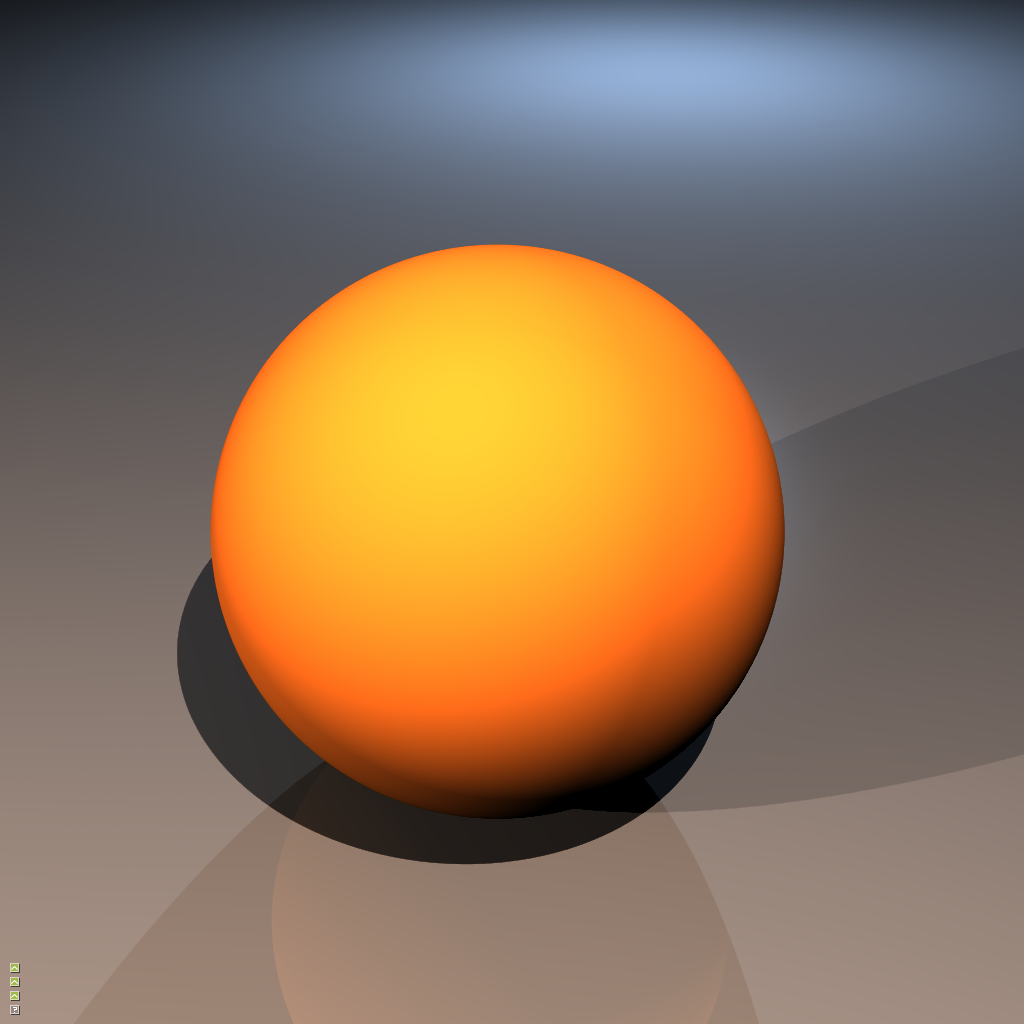
\includegraphics[width=0.2\linewidth]{../sopro/phong/phongdiff10}
\end{center}
\end{frame}



\subsection{Phong}
\begin{frame}[allowframebreaks]
\frametitle{Phong}

\begin{itemize}
\item nach [Pho75]
\item einfaches und erstes empirisches standard Modell für glänzende Oberflächen(Kunststoff)
\end{itemize}


\begin{equation}
K_d = \frac{\rho_d}{\pi}
\end{equation}
\begin{equation}
K_s = \rho_s \cdot \frac{s+2}{2\pi} \cdot cos^s\psi
\end{equation}

\begin{table}[H]
\begin{tabular}{| c | l |}
\hline
$\rho_d$ & Parameter : diffuse coefficient\\ \hline
$\rho_s$ & Parameter : specular coefficient\\ \hline
$s$ & Parameter : shiny exponent, controls roughness\\ \hline
$cos\psi$ & angle between outgoing and reflected ray\\ \hline
\end{tabular}
\end{table}

\framebreak
\begin{figure}[H]
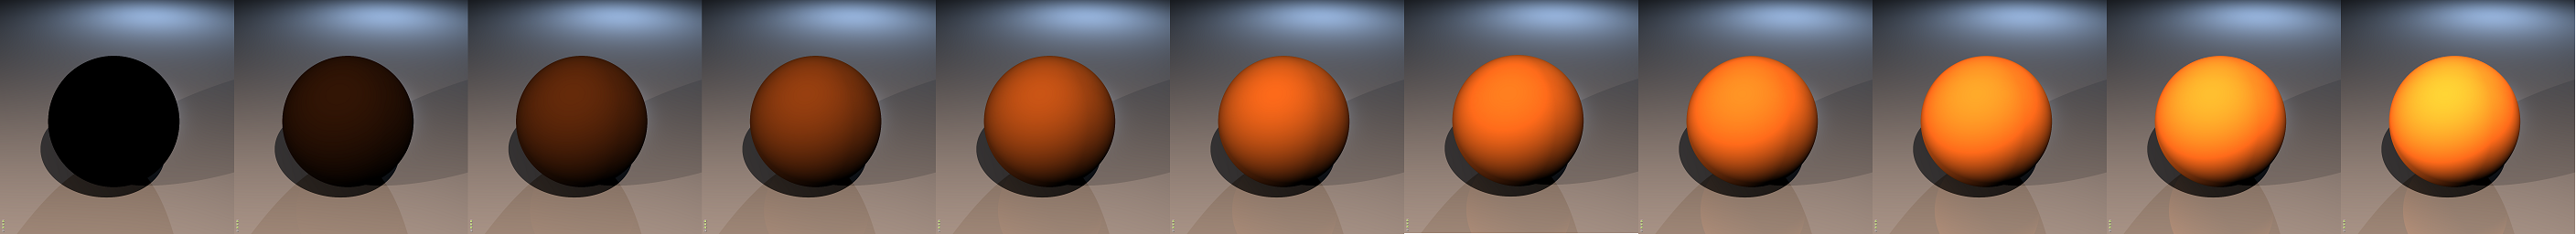
\includegraphics[width=\textwidth]{../phongdiffcomplete}
\caption{Parameter $\rho_d$ from $0.0$ to $1.0$}
\end{figure}

\begin{figure}[H]
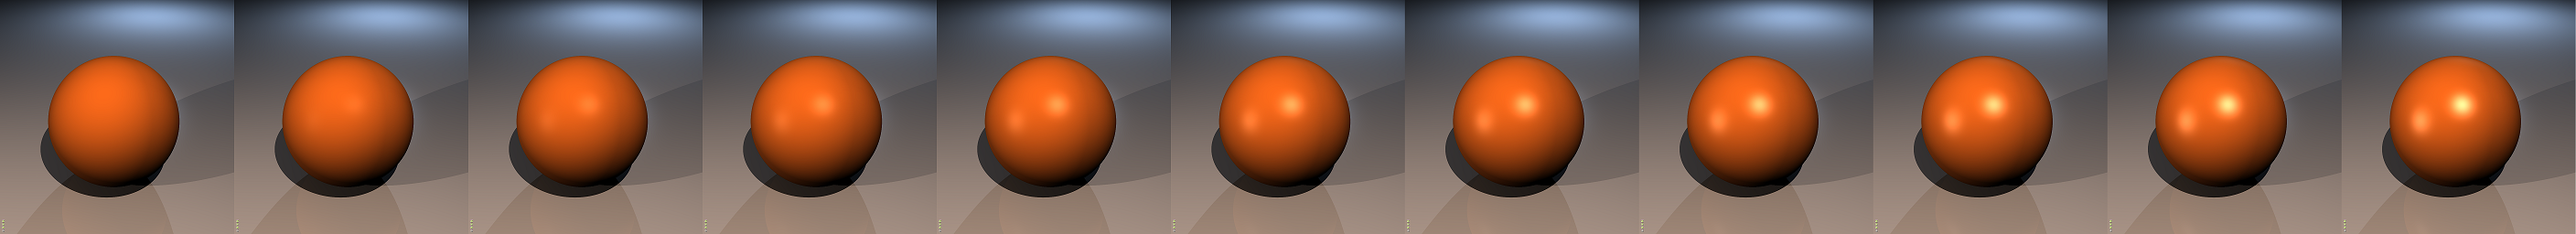
\includegraphics[width=\textwidth]{../phongspeccomplete}
\caption{Parameter $\rho_s$ from $0.0$ to $1.0$}
\end{figure}

\begin{figure}[H]
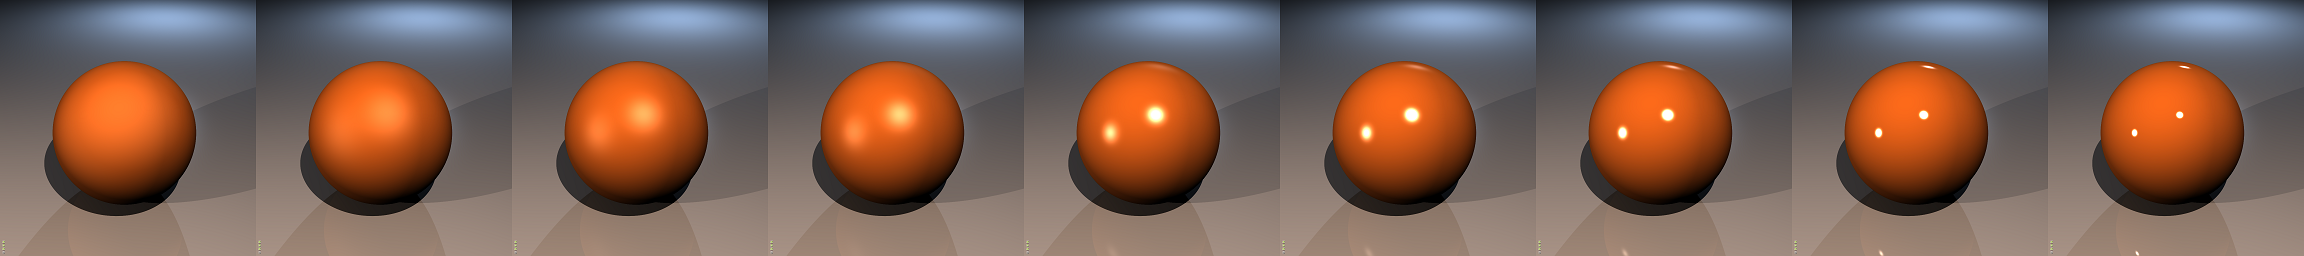
\includegraphics[width=\textwidth]{../phongshinecomplete}
\caption{Parameter $s$ from $1$ to $1000$}
\end{figure}

\begin{figure}[H]
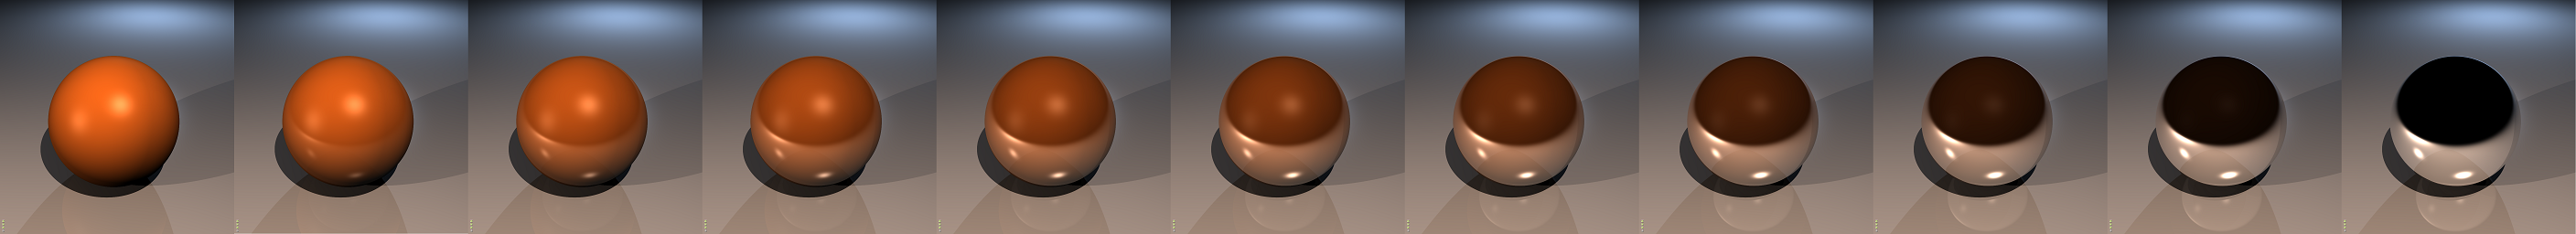
\includegraphics[width=\textwidth]{../phongreflcomplete}
\caption{Parameter $\delta$ from $0.0$ to $1.0$}
\end{figure}

\end{frame}



\subsection{Blinn Phong}
\begin{frame}[allowframebreaks]
\frametitle{Blinn Phong}
\begin{itemize}
\item nach [Bli77]
\item erweitert das standard Phong-Modell um den Halbvektor $\vec{H}$
\end{itemize}

\begin{equation}
K_d = \frac{\rho_d}{\pi}
\end{equation}
\begin{equation}
K_s = \rho_s \cdot \frac{s+8}{8\pi} \cdot cos^s\psi
\end{equation}

\begin{table}[H]
\begin{tabular}{| c | l |}
\hline
$\cos\psi$ & angle between outgoing ray and half vector $\vec{H}$\\ \hline
\end{tabular}
\end{table}
\begin{equation}
\vec{H} = \frac{\vec{L}+\vec{V}}{length(\vec{L}+\vec{V})}
\end{equation}

\begin{figure}[H]
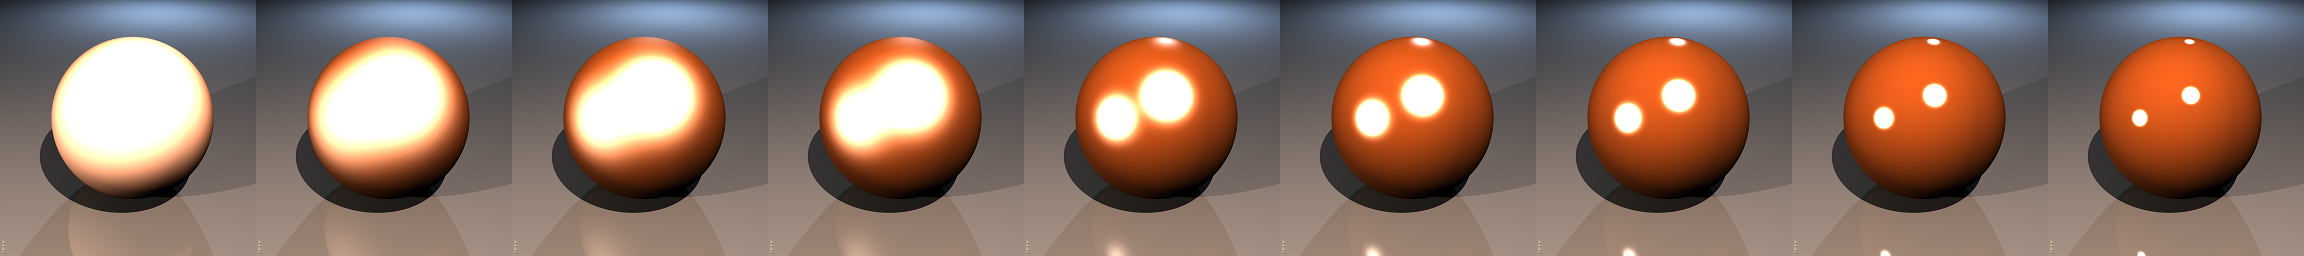
\includegraphics[width=\textwidth]{../blinnphongshinecomplete}
\caption{Parameter $s$ from $1$ to $1000$}
\end{figure}

\end{frame}



\subsection{Cook Torrance}
\begin{frame}[allowframebreaks]
\frametitle{Cook Torrance}

\end{frame}



\subsection{Ward}
\begin{frame}[allowframebreaks]
\frametitle{Ward}

\end{frame}



\subsection{Ashikhmin Shirley}
\begin{frame}[allowframebreaks]
\frametitle{Ashikhmin Shirley}

\end{frame}



\subsection{Glas}
\begin{frame}[allowframebreaks]
\frametitle{Glas}

\end{frame}



\section{Ergebnisse}
\begin{frame}[allowframebreaks]
\frametitle{Ergebnisse}

\end{frame}



\section{Demo}
\begin{frame}[allowframebreaks]
\frametitle{Demo}

\end{frame}


\end{document}